\chapter{Trabajo Futuro}
El sistema de gestión financiera personal desarrollado en el presente trabajo terminal fue concluido satisfactoriamente, cumpliendo con los objetivos planteados en la primera etapa del proyecto. La plataforma web, la aplicación móvil y el backend se encuentran funcionales e integrados, contando además con un módulo de reconocimiento óptico de caracteres que combina procesamiento local con servicios de visión artificial externos para garantizar una extracción de datos confiable incluso en condiciones adversas de captura.

\bigskip

No obstante, durante el desarrollo se identificaron funcionalidades que, por restricciones de tiempo propias del alcance del trabajo terminal, no pudieron ser incorporadas en esta versión, pero que representan oportunidades de mejora relevantes para iteraciones futuras del sistema.

\bigskip

En primer lugar, se contempla la implementación de \textbf{planes financieros compartidos}, que permitan a parejas o grupos de convivencia gestionar sus finanzas de manera conjunta dentro de la misma plataforma, con vistas diferenciadas por usuario y consolidadas por grupo. Esta funcionalidad ampliaría considerablemente el alcance de la aplicación hacia nuevos perfiles de usuario.

\bigskip

En segundo lugar, se propone la incorporación de \textbf{registro de gastos e ingresos por voz}, permitiendo al usuario dictar el concepto y el monto de un movimiento sin necesidad de interactuar con la pantalla. Esta funcionalidad, apoyada en las APIs de reconocimiento de voz disponibles en Flutter, reduciría la fricción del registro en situaciones donde el uso táctil resulta poco práctico —como al conducir o al salir de una tienda— y complementaría de forma natural el flujo de escaneo de tickets ya existente.

\bigskip

Asimismo, se considera la \textbf{integración con Google Identity} para el inicio de sesión y la validación de cuentas de usuario. Esta integración reduciría la fricción en el proceso de registro, mejoraría la seguridad mediante autenticación delegada y es coherente con las tecnologías ya empleadas en el stack actual, particularmente en el frontend desarrollado con React y en la aplicación móvil construida con Flutter.

\bigskip

Por otro lado, se plantea la \textbf{publicación de la aplicación móvil en la Google Play Store y la App Store}, lo cual requeriría atravesar los procesos de revisión y certificación correspondientes, así como ajustes en materia de políticas de privacidad y manejo de datos financieros del usuario. Este paso convertiría al sistema en un producto accesible al público general y no únicamente a usuarios de entornos de prueba.

\bigskip

finalmente, dado que el módulo de OCR demostró métricas satisfactorias de precisión pero delega a servicios externos los casos de mayor dificultad, se contempla como trabajo futuro la \textbf{exploración de modelos de reconocimiento especializados en documentos fiscales mexicanos}, tales como tickets de punto de venta y facturas electrónicas, con el objetivo de reducir la dependencia de servicios de terceros y optimizar los tiempos de procesamiento en escenarios de alto volumen.

\subsection*{Cronogramas del Trabajo Terminal}

\begin{figure}[H]
    \centering
    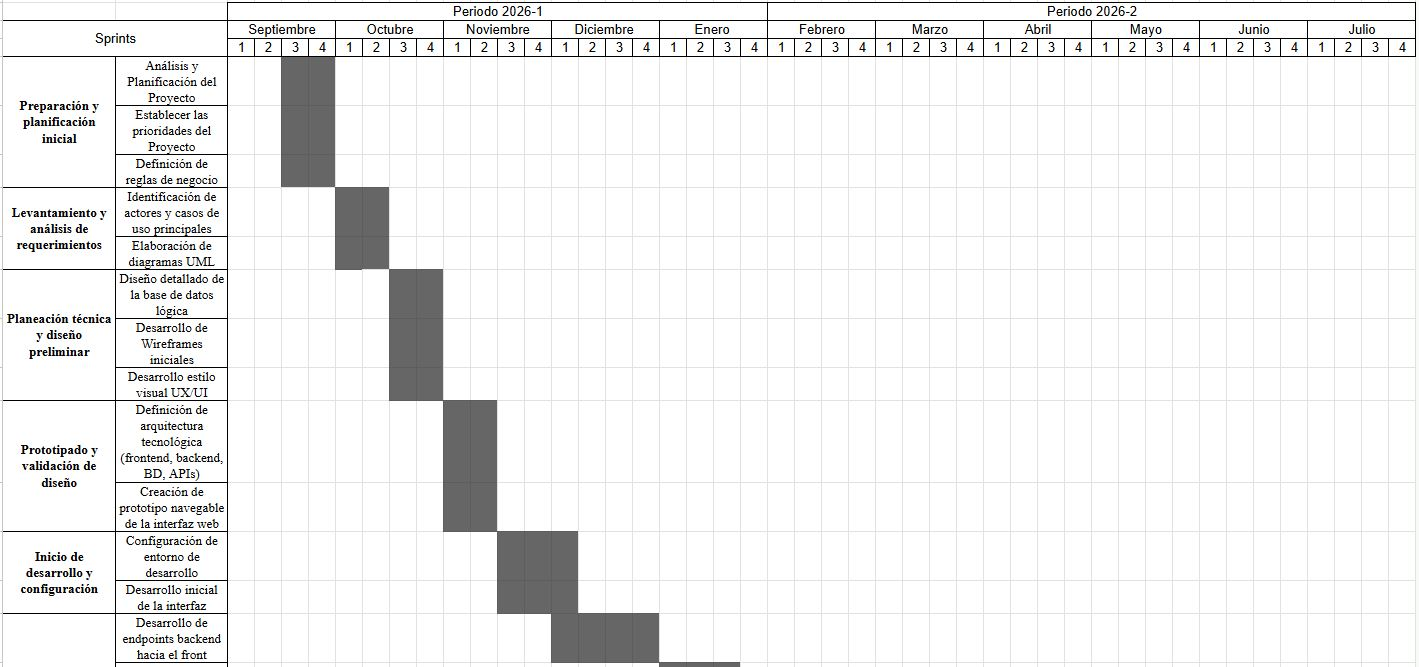
\includegraphics[width=1\linewidth]{./images/CronogramaArmando1.JPG}
    \caption{Cronograma Pt.1 Acevedo Martinez Armando - Trabajo Futuro}
\end{figure}

\begin{figure}[H]
    \centering
    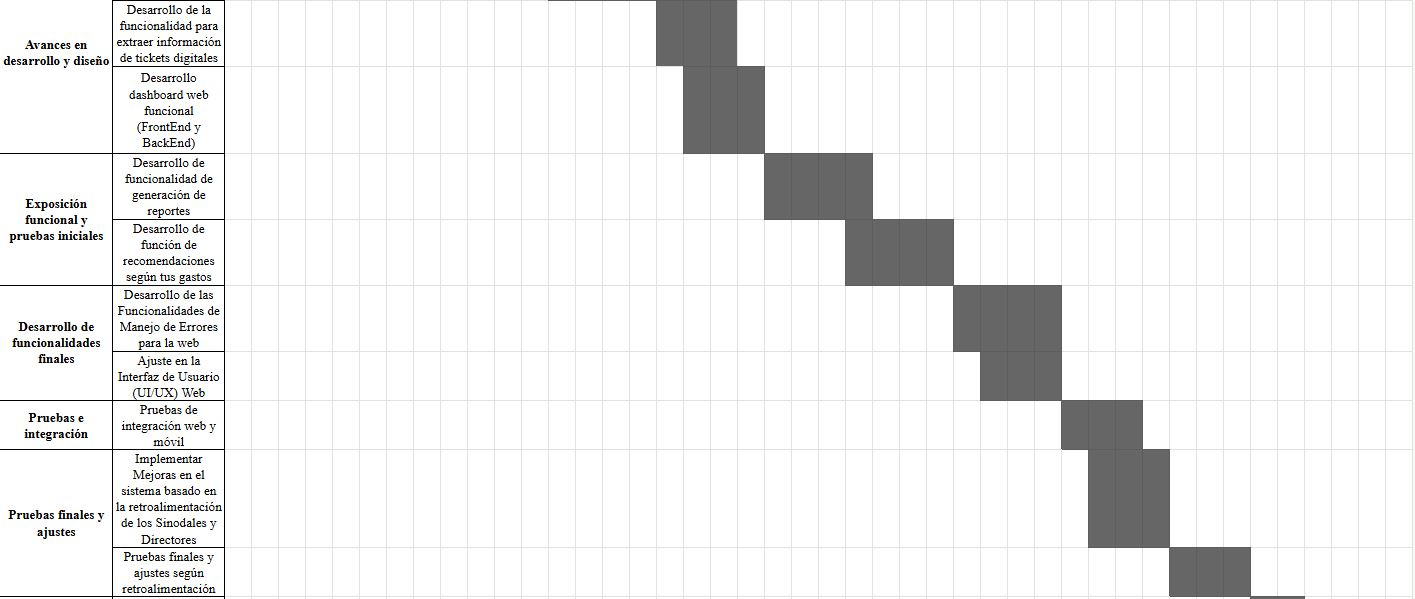
\includegraphics[width=1\linewidth]{./images/CronogramaArmando2.JPG}
    \caption{Cronograma Pt.2 Acevedo Martinez Armando - Trabajo Futuro}
\end{figure}

\begin{figure}[H]
    \centering
    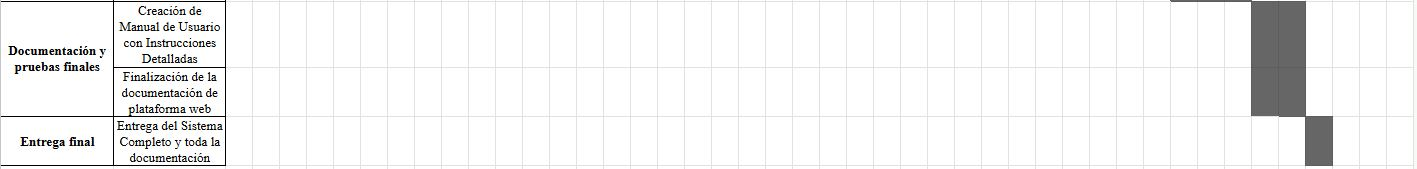
\includegraphics[width=1\linewidth]{./images/CronogramaArmando3.JPG}
    \caption{Cronograma Pt.3 Acevedo Martinez Armando - Trabajo Futuro}
\end{figure}

\begin{figure}[H]
    \centering
    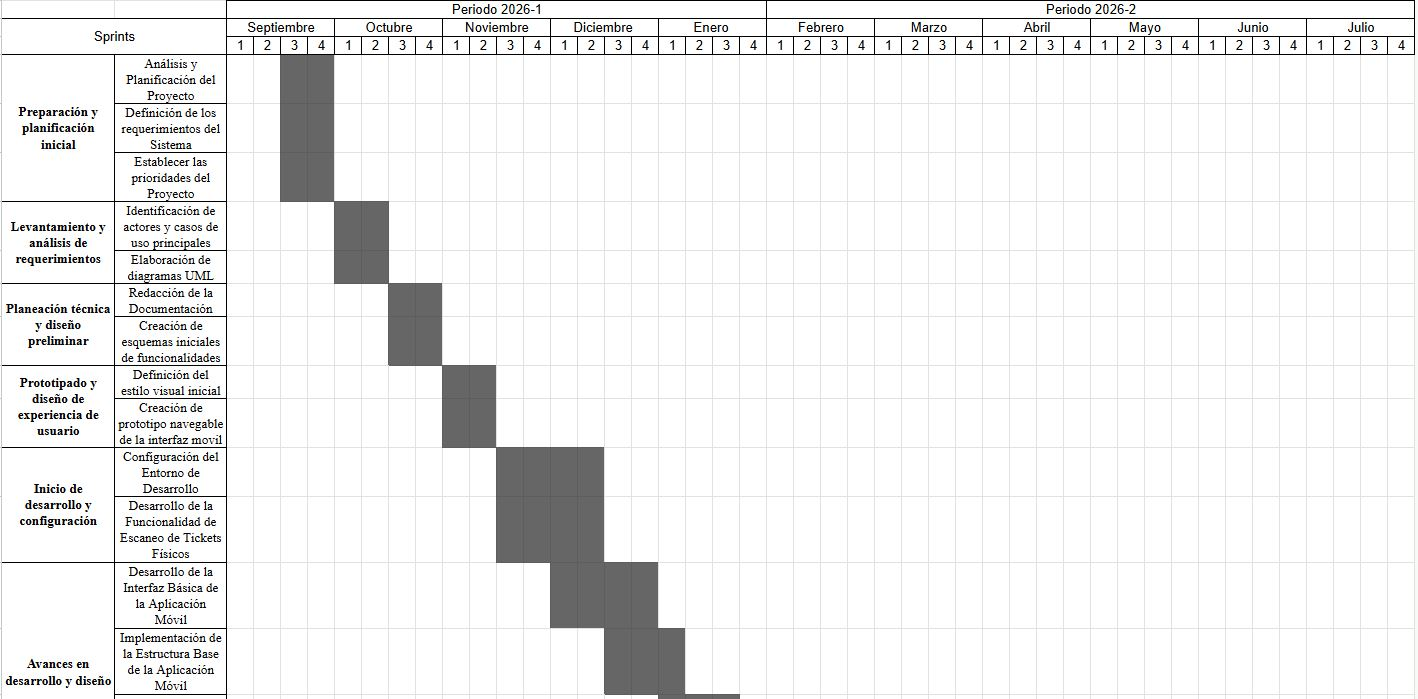
\includegraphics[width=1\linewidth]{./images/CronogramaJesus1.JPG}
    \caption{Cronograma Pt.1 Cadenas Acevedo Jesus Alejandro - Trabajo Futuro}
\end{figure}

\begin{figure}[H]
    \centering
    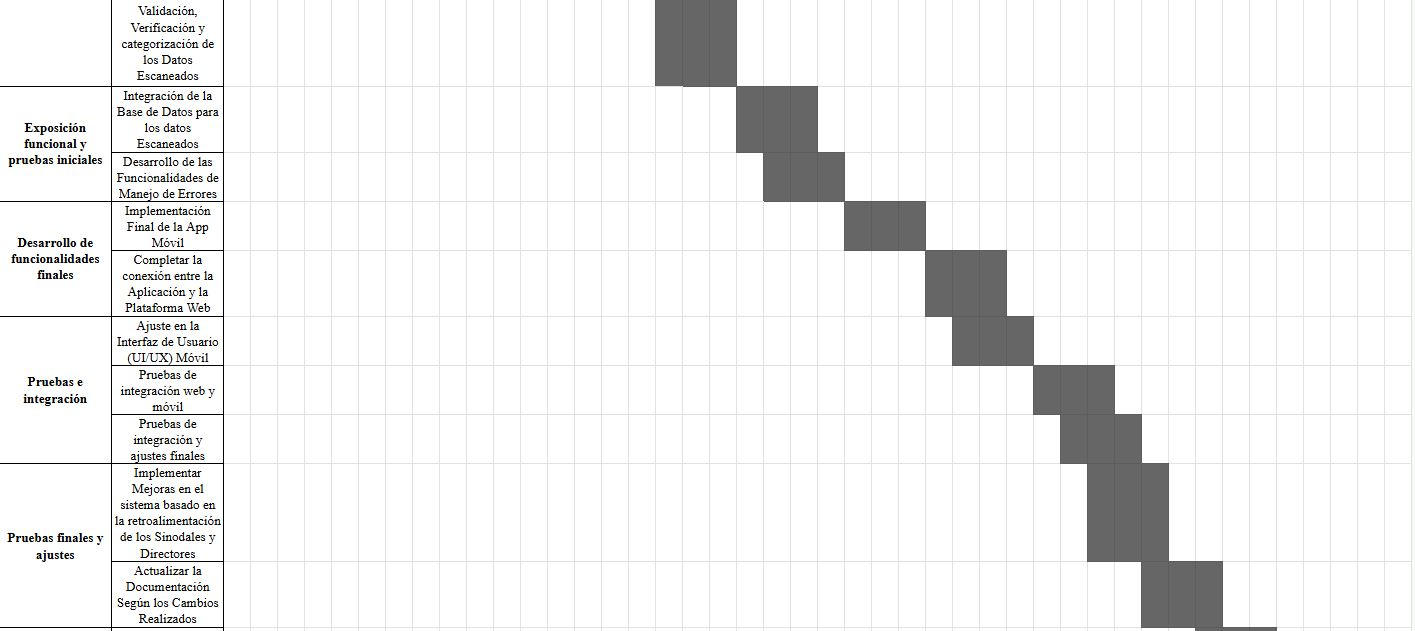
\includegraphics[width=1\linewidth]{./images/CronogramaJesus2.JPG}
    \caption{Cronograma Pt.2 Cadenas Acevedo Jesus Alejandro - Trabajo Futuro}
\end{figure}

\begin{figure}[H]
    \centering
    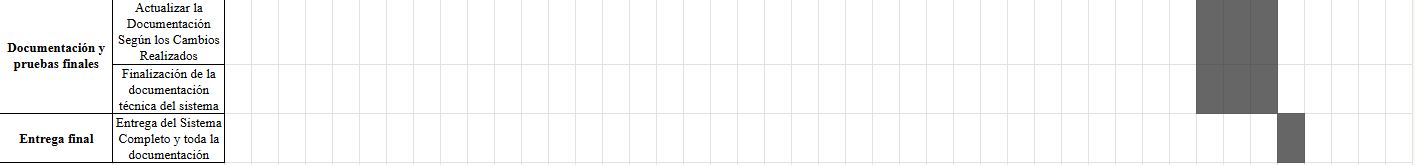
\includegraphics[width=1\linewidth]{./images/CronogramaJesus3.JPG}
    \caption{Cronograma Pt.3 Cadenas Acevedo Jesus Alejandro - Trabajo Futuro}
\end{figure}